% CAP 2
\chapter{Fundamento teórico}
Este capítulo presenta ...

\section{Elemento teórico A}
Un sistema A ...

Los elementos de ... son:
\begin{itemize}
\item{Unidad de procesamiento}
\item{Elemento de almacenamiento de datos}
\item{Dispositivos de entrada y salida}
\end{itemize}

La figura \ref{esquema_gral_plat_hw} muestra un esquema detallado con las características comúnmente observadas en estos sistemas. En esta figura se observa la unidad central de procesamiento, la memoria como elemento de almacenamiento y los periféricos como dispositivos de entrada/salida. También se puede observar el modelo híbrido para una arquitectura tipo Harvard dónde los buses para la memoria, las unidades de co-procesamiento, y los periféricos están separados.

\begin{figure}[p]
  \centering
  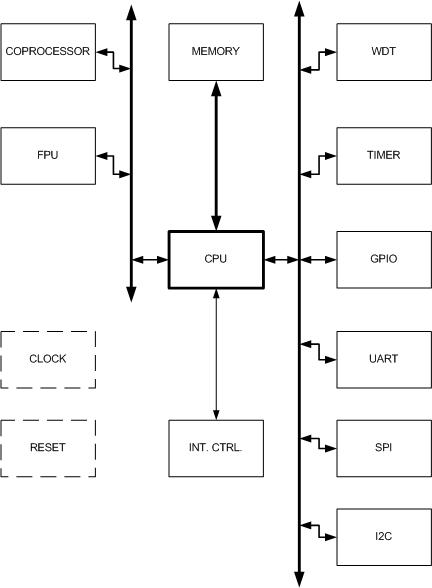
\includegraphics[width=12cm]{fig/ARQ_SE_DETALLE_1.jpg} 
  \caption[Esquema general de una plataforma hardware.]%
  {Esquema general de una plataforma hardware.}
  \label{esquema_gral_plat_hw}
\end{figure}


\subsection{Teoria A.i}
Las unidades de procesamiento usadas en... estos lenguajes son usados para describir modelos de comportamiento y son mostrados en la tabla \ref{tabla_hdls}.

\begin{table}[ht]
\begin{center}
  \begin{tabular}{|l|p{9cm}|}
    \hline
    Nombre		& Descripción \\
    \hline
    ABEL		& Advanced Boolean Expression Language, adquirido por Xilinx \\
    \hline
    AHDL		& Altera HDL. Lenguaje propietario desarrollado por Altera Corporation \\
    \hline
    Handel-C		& HDL compatible con C \\
    \hline
    MyHDL		& HDL basado en Python \\
    \hline
    SystemC		& Conjunto estandarizado de bibliotecas de clases para C++ para diseño hardware \\
    \hline
    SystemVerilog	& Un superconjunto de Verilog destinado a mejorar el proceso de diseño y verificación de sistemas \\
    \hline
    Verilog		& HDL ampliamente utilizado en el desarrollo de sistemas \\
    \hline
    VHDL		& VHSIC HDL \\
    \hline
  \end{tabular}
 \end{center}
 % \caption[SHORT]{TITLE}
 \caption[Lenguajes HDL para descripción comportamental de sistemas]{Lenguajes HDL para descripción comportamental de sistemas.}
 \label{tabla_hdls}
\end{table}

\nomenclature{ABEL}{Advanced Boolean Expression Language\\(\textsl{Lenguaje avanzado de expresiones boleanas})}%[lenguaje de descripción hardware}
\nomenclature{AHDL}{Altera HDL}
\nomenclature{Hard Processor}{\textsl{Circuito integrado que contiene un procesador}}
\nomenclature{Soft Processor}{\textsl{Procesador sintetizado en un dispositivo reconfigurable}}
\nomenclature{HDL}{Hardware Description Language \\(\textsl{Lenguaje de descripción hardware}) } % (lenguaje de descripción hardware)}
\nomenclature{VHDL}{VHSIC Hardware Description Language\\(\textsl{Lenguaje de descripción hardware para circuitos integrados de muy alta velocidad})}
% \nomenclature{VHSIC}{Very High Speed Integrated Circuit\\(\textsl{Circuito integrado de muy alta velocidad})}
\nomenclature{Verilog}{Lenguaje de descripción hardware}

\subsubsection{Teoría A.i.1}
Los procesadores ...

\paragraph{Texto énfasis.} Este texto es un ejemplo para el contenido de un párrafo

